\chapter{प्रकृति की देखभाल}\label{ch:g2:caring-for-nature}

पिकनिक के बाद एक परिवार मैदान को ठीक वैसा ही छोड़ जाता है जैसा उसे मिला
था; दूसरा थैले, बोतलों के ढक्कन और एक रौंदी हुई चींटी-बाँबी छोड़ जाता
है। मैदान के ख़रगोश, चींटियाँ और गुलबहार हमसे सँभलकर चलने को नहीं कह
सकते --- पर वे हमारी ही जगहों में साझा रहते \omterm{def:g1:living-or-not:living}{सजीव} हैं, और \omterm{def:g2:caring-for-nature:environment}{प्रकृति} में
हमारा बरताव उनके लिए मायने रखता है। \omterm{def:g2:caring-for-nature:environment}{प्रकृति} की देखभाल कोई भी, किसी भी
उम्र में सीख सकता है।

\section{प्रकृति वह है जहाँ सजीव रहते हैं}

\begin{definition}[प्रकृति और पर्यावरण]\label{def:g2:caring-for-nature:environment}
\emph{प्रकृति}\index{प्रकृति} सजीवों और उनके चारों ओर की दुनिया है:
मैदान, जंगल, तालाब, समुद्र --- और वह हवा, पानी तथा मिट्टी जिन पर वे
निर्भर हैं। जिन चीज़ों पर कोई \omterm{def:g1:living-or-not:living}{सजीव} निर्भर रहता है, उन्हें उसका
\emph{पर्यावरण}\index{पर्यावरण} कहते हैं।
\end{definition}

\begin{example}[हर चीज़ किसी न किसी का घर है]\label{ex:g2:caring-for-nature:home}
जंगल में गलता हुआ लट्ठा कचरे जैसा दिखता है --- असल में वह महल है: छाल
के नीचे भृंग, उसके नीचे कठ-जूएँ, ऊपर मॉस, और खोखल में सर्दी बिताता एक
साही। मज़े के लिए उसे तोड़ दो और चार घरानों का घर उजड़ जाता है।
\omterm{def:g2:caring-for-nature:environment}{प्रकृति} में लगभग हर चीज़ किसी न किसी का घर, भोजन या ओट है।
\end{example}

\begin{omfigure}
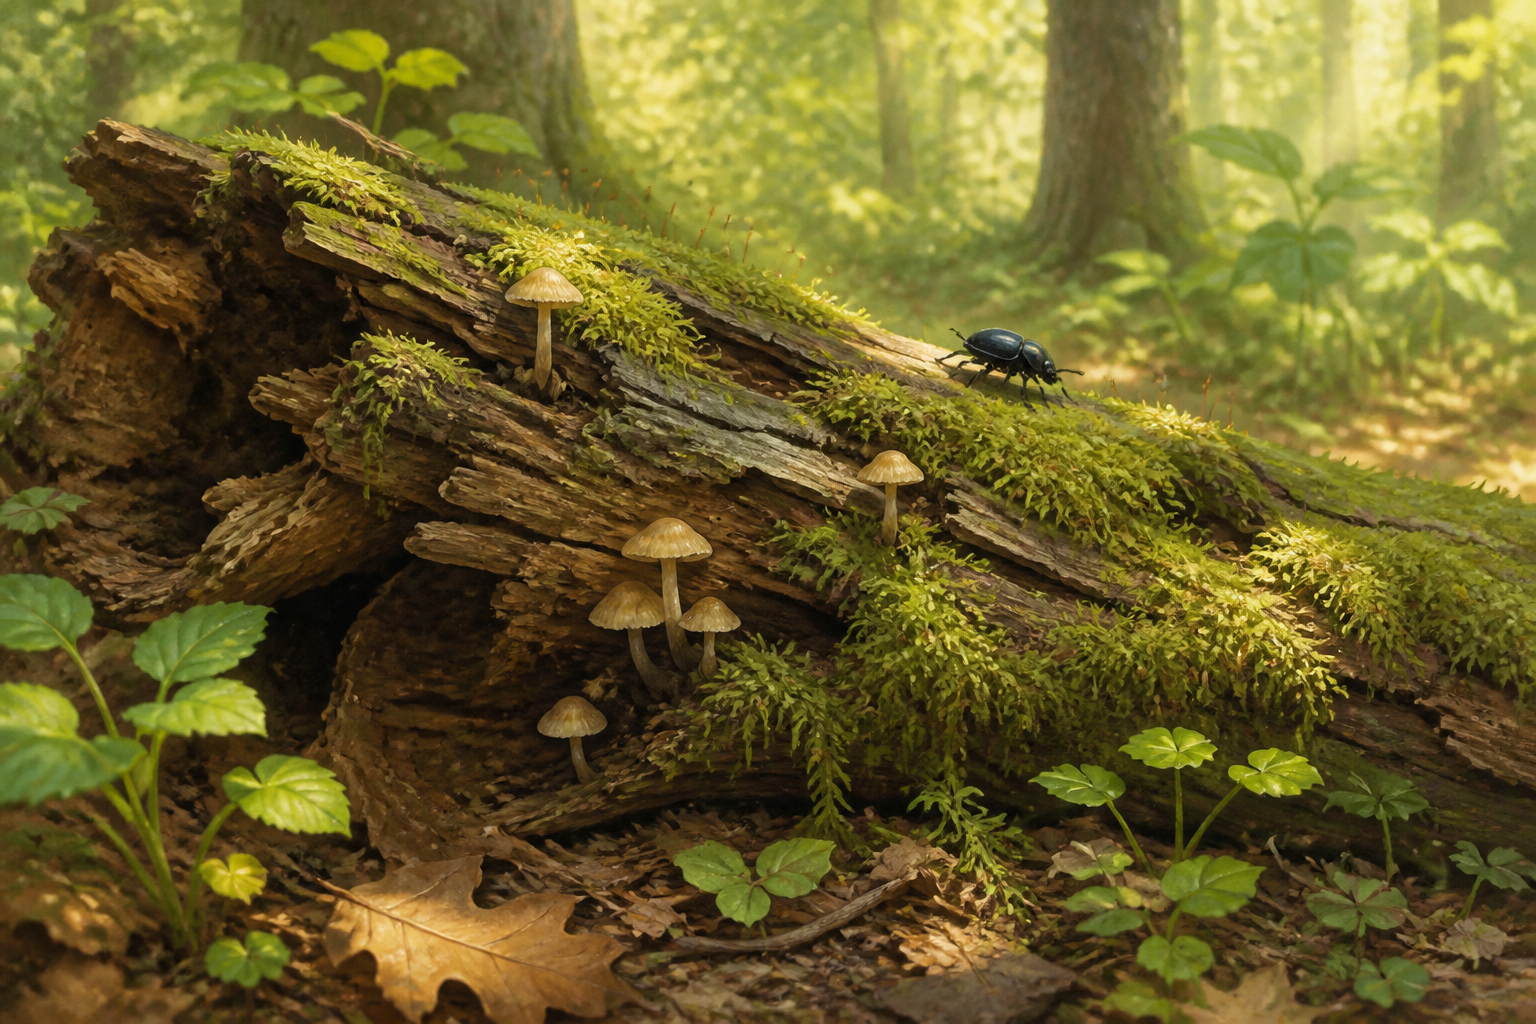
\includegraphics[width=0.62\linewidth]{images/book1/ai/g2-nature-log.png}

{\small गलता हुआ लट्ठा जो सचमुच एक महल है: छत पर मॉस, दीवारों पर
कुकुरमुत्ते, गलियारे में एक भृंग।}
\end{omfigure}

\begin{remark}[हम भी इसका हिस्सा हैं]\label{rem:g2:caring-for-nature:part}
लोग भी \omterm{def:g1:living-or-not:living}{सजीव} हैं: जो हवा हम साँस में लेते हैं, जो पानी हम पीते हैं और
जो भोजन हम खाते हैं, सब \omterm{def:g2:caring-for-nature:environment}{प्रकृति} से आता है। उसकी देखभाल सिर्फ़ ख़रगोशों
पर दया नहीं है --- वह उस दुनिया की सँभाल है जिससे हम ख़ुद जीते हैं,
जैसा \cref{ch:g2:where-animals-live} ने हर \omterm{def:g2:where-animals-live:habitat}{आवास} के बारे में कहा था।
\end{remark}

\section{क्या नुक़सान करता है, क्या मदद}

\begin{proposition}[छोटी हरकतें, सचमुच का नुक़सान]\label{prop:g2:caring-for-nature:harm}
\omterm{def:g2:caring-for-nature:environment}{प्रकृति} में नुक़सान बुरा बनने की चाह से कम ही आता है --- वह न सोचने से
आता है:
\begin{itemize}
  \item कूड़ा सालों पड़ा रहता है और \omterm{def:g1:animals-around-us:animal}{जंतुओं} को फँसा या ज़हर दे सकता है;
  \item हर \omterm{def:g1:plants-around-us:parts}{फूल} तोड़ लेने पर \omterm{def:g2:from-seed-to-plant:seed}{बीज} बनाने के लिए एक भी नहीं बचता --- और न
        मधुमक्खियों के लिए;
  \item ज़ोर से चिल्लाना और पीछे भागना \omterm{def:g1:animals-around-us:animal}{जंतुओं} को उनके भोजन और उनके
        बच्चों से दूर भगा देता है;
  \item रौंदे हुए किनारे, उलटे हुए पत्थर और टूटी हुई शाखाएँ, हर एक
        किसी छोटे घर को उजाड़ देती है।
\end{itemize}
\end{proposition}
\admitted

\begin{example}[बोतल का ढक्कन]\label{ex:g2:caring-for-nature:cap}
गिरा हुआ प्लास्टिक का ढक्कन हमारे लिए कुछ भी नहीं है और मैदान में
सालोंसाल पड़ा रहता है --- इतने सालों तक कि आज के बड़ों के बच्चे वही
ढक्कन पाएँ। \omterm{def:g2:caring-for-nature:environment}{प्रकृति} के पास कूड़ा उठाने वाली गाड़ी नहीं है: हम जो छोड़
जाते हैं, वह पड़ा रह जाता है।
\end{example}

\begin{method}[मेहमान के नियम]\label{met:g2:caring-for-nature:rules}
\omterm{def:g2:caring-for-nature:environment}{प्रकृति} में जाओ तो:
\begin{enumerate}
  \item अपना सारा कूड़ा घर ले जाओ --- पूरा का पूरा;
  \item \omterm{def:g1:plants-around-us:parts}{फूल}, कीट और घोंसले इकट्ठा करने के बजाय उन्हें देखो; ज़्यादा
        से ज़्यादा कुछ आम \omterm{def:g1:plants-around-us:parts}{फूल} तोड़ो, किसी झुरमुट के सारे कभी नहीं;
  \item जो भी पत्थर या लट्ठा तुम उलटो, उसे वापस रख दो --- उसके नीचे
        कोई रहता है;
  \item नदी-किनारों जैसी नाज़ुक जगहों के पास पगडंडी पर ही चलो;
  \item \omterm{def:g1:animals-around-us:animal}{जंतुओं} को दूर से, चुपचाप देखो, और उनके बच्चों को छोड़ दो।
\end{enumerate}
जगह ऐसी छोड़ो कि कोई बता ही न सके कि तुम वहाँ थे।
\end{method}

\begin{example}[जानबूझकर मदद करना]\label{ex:g2:caring-for-nature:help}
देखभाल नुक़सान न पहुँचाने से आगे भी जा सकती है। लू के दिनों में पानी
की एक तश्तरी, बग़ीचे का एक छोटा जंगली कोना जिसे काटा न जाए, ठंड में
पक्षियों के लिए \omterm{def:g2:from-seed-to-plant:seed}{बीज}, या
\cref{ex:g2:where-animals-live:schoolpond} जैसा स्कूल का तालाब: इनमें
से हर एक कुछ सजीवों को वह भोजन, पानी या घर देता है जो उन्होंने खो
दिया था।
\end{example}

\section{छाँटना और बचाना}

\begin{proposition}[कचरा वापस दिया जा सकता है]\label{prop:g2:caring-for-nature:recycle}
हम जो फेंकते हैं उसका बहुत कुछ फिर से काम आ सकता है। कचरे की
\emph{छँटाई}\index{कचरे की छँटाई} --- काँच काँच के साथ, काग़ज़ काग़ज़
के साथ, छिलके खाद में --- से बोतलें नई बोतलें बन जाती हैं और छिलके
मिट्टी, बजाय इसके कि सब कुछ ढेर होता जाए। और जो \emph{बचा} लिया जाता
है --- पानी, काग़ज़, बिजली --- वह कचरा बनता ही नहीं।
\end{proposition}
\admitted

\begin{example}[खाद का डिब्बा]\label{ex:g2:caring-for-nature:compost}
सेब के गूदे और गाजर के छिलके, खाद के डिब्बे में, धीरे-धीरे गहरी
भुरभुरी मिट्टी बन जाते हैं --- केंचुओं, कठ-जुओं और \omterm{def:g1:the-five-senses:sense}{आँखों} से न दिखने
वाले सजीवों की मदद से। अगले वसंत वही मिट्टी टमाटरों का पोषण करती है।
कुछ भी बरबाद नहीं हुआ; छिलके जीवन के चक्र में लौट गए।
\end{example}

\begin{remark}[छोटे हाथ भी गिनती में आते हैं]\label{rem:g2:caring-for-nature:count}
दाँत साफ़ करते समय नल बंद करना, काग़ज़ के दोनों तरफ़ लिखना, खाद का
डिब्बा, कूड़ा घर ले जाना: हर एक छोटी बात है, और लाखों लोग उन्हें करते
हैं --- या नहीं करते। \omterm{def:g2:caring-for-nature:environment}{प्रकृति} की देखभाल, या उसका नुक़सान, ज़्यादातर
तुम्हारे जैसे रोज़ के छोटे चुनावों में ही होता है।
\end{remark}

\section{अभ्यास}

\begin{exercise}[$\star$]\label{exo:g2:caring-for-nature:1}
किसी \omterm{def:g1:living-or-not:living}{सजीव} का \omterm{def:g2:caring-for-nature:environment}{पर्यावरण} क्या है? अपने \omterm{def:g2:caring-for-nature:environment}{पर्यावरण} की तीन ऐसी चीज़ें बताओ जो
\omterm{def:g2:caring-for-nature:environment}{प्रकृति} से आती हैं।
\end{exercise}

\begin{exercise}[$\star$]\label{exo:g2:caring-for-nature:2}
गलते हुए लट्ठे को तोड़ देने पर किसका घर उजड़ सकता है?
\cref{ex:g2:caring-for-nature:home} से तीन बाशिंदों के नाम बताओ।
\end{exercise}

\begin{exercise}[$\star$]\label{exo:g2:caring-for-nature:3}
\cref{met:g2:caring-for-nature:rules} के मेहमान वाले चार नियम बताओ।
\end{exercise}

\begin{exercise}[$\star$]\label{exo:g2:caring-for-nature:4}
कूड़ा हमारे साथ घर क्यों जाना चाहिए?
\cref{ex:g2:caring-for-nature:cap} के बोतल के ढक्कन से उत्तर दो।
\end{exercise}

\begin{exercise}[$\star$]\label{exo:g2:caring-for-nature:5}
किसी झुरमुट के सारे \omterm{def:g1:plants-around-us:parts}{फूल} क्यों नहीं तोड़ने चाहिए?
\cref{prop:g2:caring-for-nature:harm} के दोनों कारण बताओ।
\end{exercise}

\begin{exercise}[$\star$]\label{exo:g2:caring-for-nature:6}
खाद के डिब्बे में सेब के गूदों का क्या होता है? काम कौन करता है, और
अंत में हमें क्या मिलता है?
\end{exercise}

\begin{exercise}[$\star$]\label{exo:g2:caring-for-nature:7}
\cref{ex:g2:caring-for-nature:help} से \omterm{def:g2:caring-for-nature:environment}{प्रकृति} की जानबूझकर मदद करने
के दो तरीक़े बताओ।
\end{exercise}

\begin{exercise}[$\star$]\label{exo:g2:caring-for-nature:8}
करके देखो: अगली सैर पर दिखने वाले कूड़े के टुकड़े गिनो (ख़तरनाक टुकड़ों
को छुए बिना)। कौन-सी क़िस्म सबसे आम है? हर क़िस्म को कहाँ जाना चाहिए
था?
\end{exercise}

\begin{exercise}[$\star\star$]\label{exo:g2:caring-for-nature:9}
तालाब पर एम्मा तीन \omterm{ex:g2:animals-grow-up:frog}{टैडपोल} एक मरतबान में घर ले जाना चाहती है, ``ताकि वे
सुरक्षित बड़े हो सकें''। इस अध्याय और \cref{exo:g2:where-animals-live:10}
की मदद से बताओ कि तुम इसकी जगह क्या सलाह दोगे।
\end{exercise}

\begin{exercise}[$\star\star$]\label{exo:g2:caring-for-nature:10}
``एक बोतल का ढक्कन कुछ भी नहीं है।''
\cref{rem:g2:caring-for-nature:count} से उत्तर दो: जब दस लाख सैलानी
यही वाक्य सोचें तो क्या होता है --- ग़लत दिशा में, और सही दिशा में?
\end{exercise}
